%%%%%%%%%%%%%%%%%%%%%%%%%%%%%%%%%%%%%%%%%%%%%%%%%%%%%%%%%%%%%%%%%%%%%%%%%%%%%%%%
\section{Cadência}
\label{sec:Cadencia}
\index{Música!Cadência}

\begin{tcbinformation}{Música cadenciosa}
\index{Música!Música cadenciosa}
\label{ref:musicacadenciosa}
É aquela que tem um ritmo facilmente apreciável e que as terminações, é dizer cadencias,
são fáceis de perceber \cite[pp. 60]{pedrell2009diccionario},
Para que uma música seja cadenciada é preciso que ritmo e harmonia se combinem, 
para dar uma sensação de exatidão \cite[pp. 68]{melcior1859diccionario}.
\end{tcbinformation} 


O final da frase musical está marcado pela cadência, 
este nome vem da palavra ``cadenza''  em italiano que significa caindo ou cessando \cite[pp. 34]{bennett1993elementos} \cite[pp. 68]{melcior1859diccionario}. 
As cadências existem nas frases melódicas ou harmônicas, 
e são identificáveis como os períodos de repouso entre as frases musicais;
estas cumprem o mesmo papel que os signos de pontuação na gramática, 
já seja como virgulas, pontos e virgulas, pontos, signos de interrogação
\cite[pp. 66,67]{melcior1859diccionario} \cite[pp. 34]{bennett1993elementos}, 
etc.


%%%%%%%%%%%%%%%%%%%%%%%%%%%%%%%%%%%%%%%%%%%%%%%%%%%%%%%%%%%%%%%%%%%%%%%%%%%%%%%%
\subsection{Cadência harmônica}
\label{sec:CadenciaHarmonica}
\index{Música!Cadência harmônica}

As cadencias harmônicas estão representadas por um par de ``acordes'', 
que são usados para finalizar uma frase musical, obtendo esta um sentido de mensagem. 

Entre os tipos de cadencias harmônicas, 
temos as que nos dão a liberdade expressar uma pausa momentânea, suspenso ou o final de uma ideia.

A Tabela \ref{tab:tiposdecadencia} mostra algumas desta opções, 
na primeira coluna temos os nomes dos tipos cadencias,
na segunda coluna temos a ordem e os graus dos acordes que são usados para gerar essa cadência,
e na terceira coluna, está a descrição de cada um dos tipos de cadência.

\begin{table}[h]
  \centering
  \begin{tabular}{|p{4cm}|l|p{8cm}|}
  \hline
  Nome & Acordes   & Analogia \\ \hline
  \hline
  Cadência perfeita & V-I       & Da sentido de algo perfeitamente acabado, 
  equivalente a um ponto final na gramática \cite[pp. 34]{bennett1993elementos}. \\ \hline
  
  Cadência plagal   & IV-I      & Da um sentido equivalente a um ponto final na gramática, 
  também é chamado de cadência do ``Amém'' 
  por seu uso em hinos religiosos \cite[pp. 34]{bennett1993elementos} \\ \hline

  Cadência imperfeita ou semicadência \cite[pp. 103]{grabner2001teoria} & ?-V    & Acontece quando se vá de um grau qualquer para finalizar na dominante (V), 
  porém é comum ver que se usam:
  I-V,II-V e IV-V. Esta cadência da à música a sensação de um final incompleto, 
  seu efeito é similar ao de uma virgula na gramática,
  \cite[pp. 34]{bennett1993elementos}. \\ \hline

  Cadência interrompida & V-($\neq$I) & Acontece quando se sugere que acontecerá uma cadencia V-I (dominante-tônica),
  porém apos V se finaliza em qualquer grau 
  diferente da \hyperref[sec:Tonica]{\textbf{tônica}}, geralmente VI,
  e dá uma sensação de surpresa e de interrupção à música; é dizer uma frase incompleta.
  \cite[pp. 35]{bennett1993elementos}. \\ \hline  
\end{tabular}
  \caption{Tipos de cadência harmônica.}
  \label{tab:tiposdecadencia}
\end{table}

\begin{example}
A Figura \ref{fig:abc-perfeita1}, mostra uma cadência perfeita, para uma tônica em acorde de dó.
A cadência da a sensação de uma frase com ponto final.
\end{example}

\begin{figure}[H]
\centering
\begin{abc}[name=abc-perfeita1,width=1.0\linewidth]
X: 1 % start of header
K: C % scale: C major
M: 2/4 %meter - compasso
V:1 %name="Pauta com clave de fá"   sname="Pauta com clave de fá"
[V:1] | [C2 E2 G2] [F2 A2 C'2]| [E2 G2 B2] [G2 B2 D'2]| [F2 A2 C'2] [G2 B2 D'2]| [C2 E2 G2] z2|
w: ~ ~ ~ ~ ~ V I
\end{abc}
\caption{Cadência perfeita.}
\label{fig:abc-perfeita1}
\end{figure}

\begin{example}
A Figura \ref{fig:abc-plagal1}, mostra uma cadência plagal, para uma tônica em acorde de dó.
A cadência da a sensação de uma frase com ponto ao  final.
\end{example}

\begin{figure}[H]
\centering
\begin{abc}[name=abc-plagal1,width=1.0\linewidth]
X: 1 % start of header
K: C % scale: C major
M: 2/4 %meter - compasso
V:1 %name="Pauta com clave de fá"   sname="Pauta com clave de fá"
%[V:1] | [E2 G2 B2] [F2 A2 C'2]| [E2 G2 B2] [G2 B2 D'2]| [C2 E2 G2] z2|
[V:1] | [C2 E2 G2] [F2 A2 C'2]| [E2 G2 B2] [G2 B2 D'2]| [E2 G2 B2] [F2 A2 C'2]| [C2 E2 G2] z2|
w: ~ ~ ~ ~ ~ IV I
\end{abc}
\caption{Cadência plagal.}
\label{fig:abc-plagal1}
\end{figure}

\begin{example}
A Figura \ref{fig:abc-imperfeita1}, mostra uma cadência imperfeita, para uma tônica em acorde de dó.
A cadência da a sensação de uma frase com um final debil, como de uma mistura de signo de admiração e interrogação.
\end{example}

\begin{figure}[H]
\centering
\begin{abc}[name=abc-imperfeita1,width=1.0\linewidth]
X: 1 % start of header
K: C % scale: C major
M: 2/4 %meter - compasso
V:1 %name="Pauta com clave de fá"   sname="Pauta com clave de fá"
[V:1] | [C2 E2 G2] [F2 A2 C'2]| [E2 G2 B2] [G2 B2 D'2]| [E2 G2 B2] [F2 A2 C'2]| [G2 B2 D'2] z2|
w: ~ ~ ~ ~ ~ IV V
\end{abc}
\caption{Cadência imperfeita.}
\label{fig:abc-imperfeita1}
\end{figure}


\begin{example}
A Figura \ref{fig:abc-interrompida1}, mostra uma cadência interrompida, para uma tônica em acorde de dó.
A cadência da a sensação de uma frase incompleta.
\end{example}

\begin{figure}[H]
\centering
\begin{abc}[name=abc-interrompida1,width=1.0\linewidth]
X: 1 % start of header
K: C % scale: C major
M: 2/4 %meter - compasso
V:1 %name="Pauta com clave de fá"   sname="Pauta com clave de fá"
[V:1] | [C2 E2 G2] [F2 A2 C'2]| [E2 G2 B2] [G2 B2 D'2]| [E2 G2 B2] [G2 B2 D'2]| [A2 C'2 E'2] z2|
w: ~ ~ ~ ~ ~ V VI
\end{abc}
\caption{Cadência interrompida.}
\label{fig:abc-interrompida1}
\end{figure}

%%%%%%%%%%%%%%%%%%%%%%%%%%%%%%%%%%%%%%%%%%%%%%%%%%%%%%%%%%%%%%%%%%%%%%%%%%%%%%%%
\subsection{Cadência melódica} 
\label{subsec:cadenciamelodica}
Quando nos referimos à forma em que uma melodia é finalizada,
estamos falando da cadencia melódica; esta pode ser categorizada em: 
\begin{itemize}
\item \textbf{Cadências}, se o repouso é equivalente a um ponto na gramática \cite[pp. 66,67]{melcior1859diccionario},
como o produzido por uma dominante (V) seguida de um tônica (I).
\item \textbf{Semicadências}, se repouso é equivalente a um ponto e virgula na gramática \cite[pp. 66,67]{melcior1859diccionario};
também é chamado de cadencia imperfeita e se carateriza por terminar em dominante (V),
que geralmente vem precedido por  I, II ou IV \cite[pp. 103]{grabner2001teoria}; 
é possível ver este tipo de cadencia no final da frase antecedente de um 
\hyperref[sec:Periodo]{\textbf{período}} \cite[pp. 21]{latham2008diccionario}.
\item \textbf{Quartos de cadência}, se o repouso é igual a uma virgula \cite[pp. 66,67]{melcior1859diccionario}.
\end{itemize}~

Todas estas cadencias dão à melodia uma sensação da conclusão de uma ideia; 
porém, cada uma destas nos deixa uma perspetiva diferente sobre o que vem depois e quando.

Além dos tipos de cadencias melódicas anteriormente mencionadas, podemos achar também a:
\begin{itemize}
\item \textbf{Cadência interrompida}, este tipo de cadencias se verificam 
quando ao final de um período sugerimos que iremos de 
\hyperref[sec:dominante]{\textbf{dominante}} a \hyperref[sec:Tonica]{\textbf{tônica}},
porém terminamos em qualquer outra; é dizer, pulamos da dominante a qualquer outro grau 
\cite[pp. 67]{melcior1859diccionario} \cite[pp. 60]{pedrell2009diccionario}. 
\end{itemize}~

Em geral veremos um uso aprimorado das cadências, na frase consequente de um \hyperref[sec:Periodo]{\textbf{período}},
onde o tipo do cadência ajudará a expressar o uso que este tera na peça musical  \cite[pp. 66,67]{melcior1859diccionario}.

\begin{example}
A Figura \ref{fig:abc-frasemelodica1} mostra duas frases com tônica em dó, 
a primeira frase com uma semicadencia (VI-V) e a segunda frase com uma cadência (V-I).
\end{example}

\begin{figure}[H]
\centering
    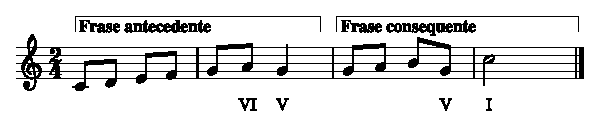
\includegraphics[width=\textwidth]{chapters/cap-musica-composer/frasemelodica1-1.eps}
\caption{Duas frases melódicas com tônica em dó.}
\label{fig:abc-frasemelodica1}
\end{figure}

\begin{example}
A Figura \ref{fig:abc-frasemelodica2} mostra duas frases  com tônica em sol, 
a primeira frase com uma cadência interrompida (V-III) e a segunda frase com uma cadência (V-I).
\end{example}

\begin{figure}[H]
\centering
    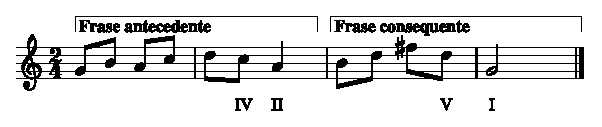
\includegraphics[width=\textwidth]{chapters/cap-musica-composer/frasemelodica2-1.eps}
\caption{Duas frases melódicas com tônica em sol.}
\label{fig:abc-frasemelodica2}
\end{figure}
% https://es.wikipedia.org/wiki/Cadencia_(música)

% https://en.wikipedia.org/wiki/Cadence

